\section{Crowdsourced-Tracking: Funktionsweise}
\label{sec:Funktionsweise}

Mit der Einführung ihres ersten \ac{BLE}-Trackers hat die Firma Tile 2013 das Konzept eines \ac{BLE}-basierten Tracking-Systems populär gemacht.
Wie viele konkurrierende Systeme, darunter Apples „Wo ist?“ Dienst, setzt auch Tile auf crowdsourcing zur Bestimmung der Position verlorener Gegenstände \cite{Weller_BLE_Finders}.
Die grundlegende Funktion dieser Systeme ist jeweils identisch und in \autoref{fig:tracker_allgemein} gezeigt: Ein zu findendes Gerät \textit{c)} sendet periodisch \ac{BLE}-Advertisements, die von Smartphones in der Nähe \textit{b)} empfangen werden \textit{(1)}.
Das zu findende Gerät ist dabei entweder ein Endgerät wie ein Smartphone oder ein Tablet, oder ein spezieller, batteriebetriebener, sogenannter Tracker.
Solche Tracker können an anderen Gegenständen befestigt werden, sodass diese bei Verlust ebenfalls gefunden werden können.
Die Empfänger der \ac{BLE}-Advertisements können ihre Position über das \ac{GPS} bestimmen und diese zusammen mit einer ID, welche das zu findende Gerät identifiziert, an einen Server übermitteln \textit{(2)}.
Der Besitzer des zu findenden Geräts, kann mit einem anderen Gerät \textit{a)} die Position vom Server abrufen \textit{(3)} \cite{Garg_Secure_Tracker}.
Das Funktionsprinzip ist dementsprechend einfach.
\begin{figure}[ht]
    \centering 
    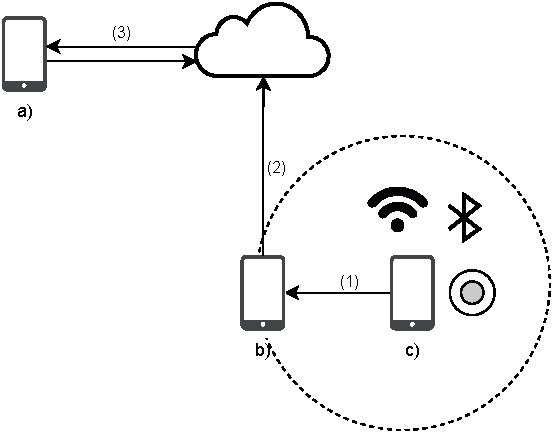
\includegraphics[width=0.6\textwidth]{BLE_Tracker_allgemein.pdf}
    \caption{Allgemeine Funktionsweise des Crowdsourced-Tracking mit \ac{BLE}.}
    \label{fig:tracker_allgemein}
\end{figure}
Qualität und Nützlichkeit für die Nutzer eines solchen Dienstes hängt aber stark von der Anzahl der Nutzer ab.
Die Position eines verlorenen Geräts kann nur vom Tracking-Dienst abgerufen werden, wenn ein Nutzer des gleichen Dienstes ein \ac{BLE}-Advertisement des verlorenen Geräts empfangen und die Position an den Dienst übermittelt hat.
Weiterhin ist die Positionsbestimmung verlorener Geräte nur durch Android-Geräte im Hintergrund möglich, da die Bluetooth und \ac{BLE} \acp{API} unter iOS keine unbeschränkte Nutzung im Hintergrund erlauben \cite{Heinrich_AirGuard}.
Damit ist die Zahl der Android-Nutzer, welche die zum Dienst gehörende App installiert haben, entscheidend für die Funktionsfähigkeit und Qualität des Dienstes. 
Je mehr (Android) Nutzer ein Dienst hat, desto größer die Wahrscheinlichkeit, dass sich einer dieser vor kurzem in der Nähe des verlorenen Geräts befand und desto wahrscheinlicher kann das verlorene Gerät gefunden werden.


Weller \textit{et al.} \cite{Weller_BLE_Finders} und Garg \textit{et al.} \cite{Garg_Secure_Tracker} untersuchten die Funktionsweise von verschiedenen auf diesem Prinzip aufbauenden Tracking-Diensten.
Dabei wurden in allen untersuchten Diensten Schwachstellen aufgedeckt, die sowohl Privatsphäre als auch Sicherheit betreffen.
Unter anderem übermittelten einige Dienste die Positionsdaten unverschlüsselt und erlaubten das unberechtigte Abrufen von personenbezogenen Daten über die Backends der Dienste.
Auch zum Veröffentlichungszeitpunkt der Arbeit von Weller \textit{et al.} \cite{Weller_BLE_Finders} waren nicht alle der erkannten Schwachstellen behoben.
Außerdem bot keiner der von Garg \textit{et al.} \cite{Garg_Secure_Tracker} untersuchten Dienste ausreichend Schutz vor dem Melden falscher Positionsdaten.


\subsection{Funktionsweise des „Wo ist?“ Dienstes im Detail}
\label{sec:Funktionsweise_FindMy}
Auf seiner Informationsseite über den „Wo ist?“ Dienst gibt Apple zur Sicherheit seines Dienstes an: „Geräte in der Nähe senden den Standort [...] sicher an iCloud weiter [...]. Zum Schutz der Privatsphäre passiert das alles anonym und verschlüsselt“ \cite{Apple_WoIst}.
Apple erhebt demnach den Anspruch einen Dienst anzubieten, der, im Vergleich zu den Diensten der Konkurrenz, nicht nur sicherer, sondern auch besser für die Privatsphäre der Nutzer ist.
Vergangene Untersuchungen haben allerdings bereits gezeigt, dass auch Apples Dienst einige Schwachstellen aufweist \cite{Heinrich_FindMy,Tonetto_FindMy}.
Diese Schwachstellen werden in \autoref{sec:Missbrauch} wieder aufgegriffen.

Der vermutlich größte Vorteil des Dienstes liegt aber in der großen Zahl der Geräte, welche aktiv die Positionsdaten verlorener Geräte sammeln.
Laut Apple nehmen „hunderte[n] Millionen iPhone, iPad und Mac Geräte[n]“ \cite{Apple_WoIst} am „Wo ist?“ Dienst teil.
Der größte Konkurrent Tile hatte im Jahr 2021, laut der bekannten Gadget-Review Webseite \textit{Pocket-Lint}, 40 Millionen Nutzer und kann damit für die Lokalisierung auf ein deutlich kleineres Netzwerk zurückgreifen als Apple \cite{Tile_Network}.
Durch die bereits beschriebene Limitierung der Hintergrundnutzung von \ac{BLE} unter iOS schränkt Apple alle Konkurrenten zusätzlich stark ein.
Der „Wo ist?“ Dienst kann hingegen standardmäßig auf alle Apple-Geräte zur Lokalisierung verlorener Geräte zurückgreifen \cite{Heinrich_AirGuard}.

Auf Basis des Reverse-Engineerings des „Wo ist?“ Dienstes von Heinrich \textit{et al.} in \cite{Heinrich_FindMy} und der Spezifikation für Drittanbieter \cite{Apple_FindMySpec}, wird im Folgenden die grundlegende Funktionsweise des Dienstes erläutert.
Dabei wird insbesondere darauf eingegangen, welche Maßnahmen Apple ergreift, um Sicherheit und Privatsphäre der Nutzer besser zu schützen als die konkurrierenden Dienste. 

Die Spezifikation definiert für den „Wo ist?“ Dienst die folgenden vier Rollen \cite{Apple_FindMySpec}:
\begin{itemize}
    \item \textbf{Owner Device}: Alle Geräte, in denen die Apple-ID des Besitzers hinterlegt ist.
    \item \textbf{Accessory}: Das zu findende Gerät. Allgemeiner auch als \textbf{Lost Device} bezeichnet.
    \item \textbf{Find My network}: Die Menge aller Apple-Geräte, mit aktivierter „Wo ist?“ Funktion. Einzelne Geräte werden jeweils als \textbf{Finder Device} bezeichnet. Diese sind für das Erstellen sogenannter \textit{Location Reports} verantwortlich.
    \item \textbf{Apple Server}: Server der die Location Reports speichert.
\end{itemize}
Die Rollen \textit{Owner Device}, \textit{Lost Device} und \textit{Finder Device} können von allen Apple-Endgeräten angenommen werden.
\textit{Accessories} stellen einen Spezialfall von Lost Devices dar.
Apple erlaubt seit April 2021 auch Drittanbietern die Nutzung des „Wo ist?“ Netzwerks zur Lokalisierung von Geräten \cite{Apple_FindMy3rdParty}.
Allgemein werden alle Geräte, die den „Wo ist?“ Dienst nutzen, und keine Internetverbindung herstellen können, als Accessories betrachtet.
Dazu gehören insbesondere Produkte von Drittanbietern und Apples AirTags.
Accessories können die anderen Rollen nicht annehmen und sind damit nur in der Lage lokalisiert zu werden, können aber die Lokalisierung anderer Geräte nicht unterstützen.
Damit sind sie im Vergleich zu Owner oder Finder Devices nur passive Teilnehmer im „Wo ist?“ Netzwerk.

Jedes Lost Device muss mit der Apple-ID des Besitzers verbunden sein und die „Wo ist?“ Funktion muss in der Apple-ID des Nutzers aktiviert sein.
Bei Endgeräten wie dem iPhone oder dem iPad wird die Apple-ID standardmäßig hinterlegt.
Bei Accessories muss ein initialer Pairing-Prozess mit einem Endgerät durchlaufen werden \cite{Apple_FindMySpec}.

\subsubsection{Kryptografie}
\label{sec:Kryptografie}
Apple verwendet asymmetrische \ac{ECC}-Verschlüsselung, um eine im Vergleich zur Konkurrenz höhere Sicherheit und besseren Schutz der Privatsphäre zu gewährleisten.
Alle Standortdaten werden mit einer Ende-zu-Ende-Verschlüsselung vor unbefugtem Zugriff geschützt.
So können weder Apple noch potenzielle Angreifer die Positionen der Nutzer auslesen.
Nur der Besitzer des Geräts kann die verschlüsselten Daten zur Lokalisierung des Geräts entschlüsseln \cite{Greenberg_FindMyCrypto}.

Um eine Ende-zu-Ende-Verschlüsselung zu ermöglichen, müssen alle Geräte eines Besitzers Zugriff auf gemeinsame Schlüssel haben.
Wie diese Schlüssel generiert und genutzt werden, wird im Folgenden erläutert.
Die Generierung ist in \autoref{fig:crypto_keygen} dargestellt.
Jedes Owner Device \textit{a)} erzeugt zunächst ein \ac{ECC}-Schlüsselpaar $K_{ECC}$ und einen symmetrischen Schlüssel $SK$ \textit{(1)}.
Diese bilden zusammen den sogenannten \textit{\ac{MBK}} ($MBK = K_{ECC} + SK$).
Die \acp{MBK} werden über den iCloud Dienst zwischen allen Geräten mit der gleichen Apple-ID synchronisiert \textit{(2)}.
Um die Schlüssel bei der Synchronisierung zu schützen, werden sie mit einem symmetrischen Schlüssel, aus der als sicher geltenden iCloud-Keychain, verschlüsselt \cite{Heinrich_FindMy,Afonin_iCloudKeychain}.
   
Accessories können ihre \acp{MBK} nicht selbst über die iCloud synchronisieren.
Beim notwendigen initialen Pairing, werden vom Accessory \textit{a')} und dem Owner Device gemeinsam $K_{ECC}$ sowie zwei symmetrische Schlüssel, in der Spezifikation als $SKN$ und $SKS$ bezeichnet, berechnet \textit{(1')} \cite{Apple_FindMySpec}.
Aus diesen Schlüsseln lassen sich zwei unterschiedliche \acp{MBK} generieren.
Abhängig vom Zustand des Accessories bildet sich der verwendete \ac{MBK} aus dem \ac{ECC}-Schlüsselpaar und einem der beiden symmetrischen Schlüsseln.
War das Gerät schon längere Zeit nicht mit einem Owner Device verbunden (sogenannter \textit{Separated State}), wird der SK\textbf{S} (\textbf{S} = Separated) als symmetrischer Schlüssel verwendet ($MBK_{separated} = K_{ECC} + SKS$).
Solange das Gerät mit einem Owner Device verbunden ist sowie kurzzeitig nach dem Verlust der Verbindung (sogenannter \textit{Nearby State}), wird stattdessen der SK\textbf{N} (\textbf{N} = Nearby) verwendet ($MBK_{nerby} = K_{ECC} + SKN$) \cite{Apple_FindMySpec}.
Beide möglichen \acp{MBK} werden verschlüsselt über den iCloud Dienst mit allen Geräten des Besitzers synchronisiert \textit{(2)}.
Anhand dieser Schlüssel können die, für die Verschlüsselung der Standortdaten verwendeten, Schlüssel berechnet werden.
Durch die Synchronisierung der Schlüssel wird ermöglicht, dass verschlüsselte Standortdaten des „Wo ist?“ Dienstes auf allen Owner Devices entschlüsselt werden können \cite{Heinrich_FindMy}.
\begin{figure}[ht]
    \centering
    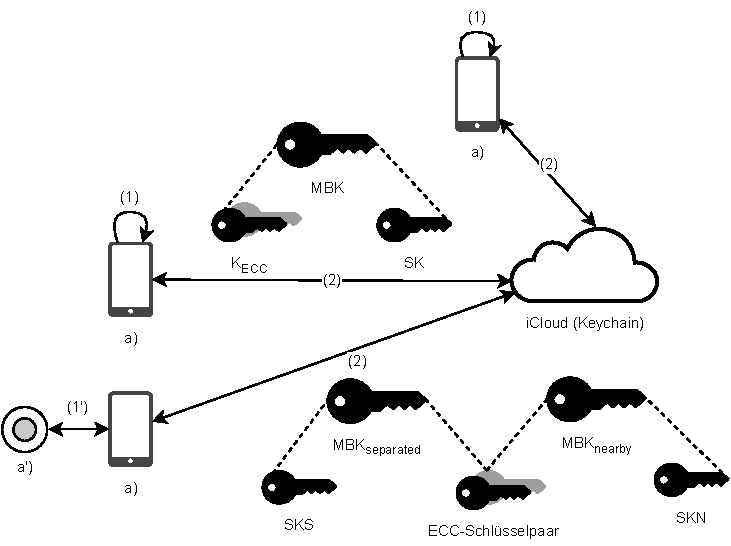
\includegraphics[width=0.9\textwidth]{krypto_keygen.pdf}
    \caption{Generierung und Synchronisierung der Master Beacon Keys.}
    \label{fig:crypto_keygen}
\end{figure}


Zur Ende-zu-Ende-Verschlüsselung der Standortdaten, wird der \ac{AES}-Algorithmus im \ac{GCM} verwendet.
Die Verschlüsselung wird dabei  auf dem Finder Device durchgeführt.
Der für die Verschlüsselung verwendete Schlüssel darf nur dem Owner Device und dem Finder Device bekannt sein.
Dazu überträgt das Lost Device in den \ac{BLE} Advertisement-Paketen einen Schlüssel, aus welchem sowohl das Finder Device als auch ein Owner Device den \ac{AES}-Schlüssel berechnen können.
Da allerdings gleichzeitig die Verfolgung eines Lost Device anhand der im Advertising übertragenen Daten nicht möglich sein soll, muss der sogenannte \textit{Advertising Key} regelmäßig gewechselt werden.
Deshalb wird die ANSI X9.63-\ac{KDF} verwendet, um temporär gültige Advertising Keys abzuleiten \cite{Apple_FindMySpec,Heinrich_FindMy}.
Ein abgeleiteter Advertising Key $AK_i$ wird jeweils für eine definierte Zeit in \ac{BLE}-Advertisement-Paketen übertragen, bevor zum nächsten Schlüssel $AK_{i+1}$ gewechselt wird.
Für die Ableitung von $AK_{i+1}$ wird neben $AK_{i}$, auch der \ac{MBK} benötigt.
Damit ist es für Außenstehende nicht möglich, den folgenden Advertising Key zu berechnen oder mehrere Advertising Keys miteinander in Verbindung zu bringen.
Durch das regelmäßige Wechseln des verwendeten Avertising Keys lässt sich verhindern, dass ein Angreifer ein Lost Device anhand der im Advertising übertragenen Daten verfolgen kann \cite{Heinrich_FindMy}.
Eine Verfolgung ist jeweils nur für das Intervall der Schlüsselrotation möglich.

Bei Accessories ist der für die Ableitung der Advertising Keys verwendete \ac{MBK} vom Zustand des Geräts abhängig.
Wie bereits beschrieben wird entweder der $MBK_{nerby}$ oder der  $MBK_{separated}$ eingesetzt \cite{Apple_FindMySpec}.
Außerdem ist das Intervall in welchem neue Advertising Keys generiert werden, abhängig vom Zustand des Geräts.
Im Separated State wird der Schlüssel dabei seltener gewechselt.
Dies ist unter anderem notwendig, um das Anti-Tracking Feature der Accessories zu ermöglichen.
Dabei erkennen Apple-Endgeräte, ob sich das gleiche Accessory längere Zeit in der Nähe befindet und können den Nutzer vor Tracking durch andere warnen.
Insbesondere mit AirTags lässt sich anderen Personen sehr einfach folgen, da diese beispielsweise leicht in Autos, Taschen oder Kleidung versteckt werden können \cite{Heinrich_AirGuard}.


Der Schlüssel für den \ac{AES}-Algorithmus wird aus dem Advertising Key $AK_i$ berechnet und muss sowohl vom Finder Device als auch vom Owner Device bestimmt werden können.
Dazu generiert das Finder Device zunächst ein temporäres \ac{ECC}-Schlüsselpaar ($K_{ECC}'$).
Über einen \ac{ECDH}-Schlüsselaustausch wird aus dem privaten Teil von $K_{ECC}'$ und dem öffentlichen Teil von $AK_i$ ein geteiltes Geheimnis ($s$) berechnet.
Durch die Anwendung der ANSI X9.63-\ac{KDF} auf $s$ wird ein symmetrischer Schlüssel $e$ generiert.
Von diesem werden die ersten 16 Byte als Schlüssel für den \ac{AES}-Algorithmus und die folgenden 16 Byte als Initialisierungsvektor verwendet \cite{Heinrich_FindMy}.
Der Prozess zur Ableitung des symmetrischen Verschlüsselungsschlüssels ist in \autoref{fig:krypto_encryption} schematisch dargestellt.
Durch die Verwendung des \ac{ECDH}-Schlüsselaustauschs kann sichergestellt werden, dass die Standortdaten nur mithilfe des privaten Teils von $AK_i$ entschlüsselt werden können.
Dieser ist nur mit Zugriff auf den \ac{MBK} des Lost Device berechenbar und kann damit nur von Owner Devices bestimmt werden \cite{Heinrich_FindMy}.

\begin{figure}[ht]
    \centering
    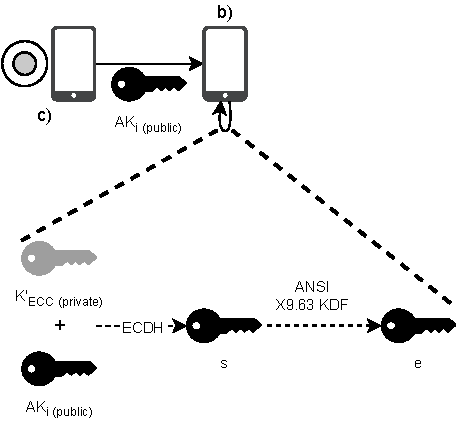
\includegraphics[width=0.6\textwidth]{krypto_encryption.pdf}
    \caption{Ableitung des \ac{AES}-Schlüssels für die Ende-zu-Ende-Verschlüsselung der Standortdaten.}
    \label{fig:krypto_encryption}
\end{figure}

Für die Entschlüsselung der Standortdaten kann $s$ über den \ac{ECDH}-Schlüsselaustausch ebenfalls mit dem öffentlichen Teil von $K_{ECC}'$ und dem privaten Teil von $AK_i$ berechnet werden.
Der symmetrische Schlüssel entsteht wieder durch die Anwendung der ANSI X9.63-\ac{KDF} auf das geteilte Geheimnis.
Damit das Owner Device diesen Prozess durchführen kann, muss der öffentliche Teil von $K_{ECC}'$ im Location Report, der von Apples Servern abgerufen wird, enthalten sein.
Außerdem muss das Owner Device erkennen können, welcher Advertising Key verwendet wurde.
Deshalb enthält jeder Location Report zusätzlich einen \ac{SHA}-256 Hashwert des öffentlichen Teils von $AK_i$.
Das Owner Device kann auf Basis des \ac{MBK} des Lost Devices so lange neue Advertising Keys ableiten, bis der Hashwert des öffentlichen Teils mit dem im Location Report enthaltenen übereinstimmt.
So kann der für die Generierung des symmetrischen Schlüssels verwendete Advertising Key bestimmt werden.
Der private Teil des Schlüssels kann dann für den Schlüsselaustausch verwendet werden \cite{Heinrich_FindMy}.


Durch die Ausführung der Verschlüsselung auf dem Finder Device, kann die Batterie des Lost Devices geschont werden und die Lokalisierung verlorener Geräte bleibt länger möglich.
Insbesondere bei AirTags oder Produkten von Drittanbietern kann das hilfreich sein, da diese Geräte eine im Vergleich zu einem iPhone oder iPad, sehr geringe Batteriekapazität haben.
Die kryptografischen Funktionen könnten den Stromverbrauch der Geräte deutlich erhöhen, wenn bei jedem Kontakt mit einem Finder-Device dieser komplexe Verschlüsselungsprozess ablaufen muss.
Insbesondere in Umgebungen mit vielen potenziellen Finder Devices wäre der Aufwand für die Verschlüsselung auf dem Lost Device sehr groß.
In einer solchen Umgebung werden vermutlich seltener neue Schlüssel abgeleitet als Finder Devices Location Reports erstellen.
Dies gilt vor allem für Accessories, welche den Schlüssel im Separated State nur alle 24 Stunden wechseln.

%TODO: continue 
\subsubsection{\ac{BLE} Advertisement des Dienstes}
\label{sec:advertisement}
Alle Apple Geräte mit aktivierter Bluetooth-Funktion, die für das Finden durch den „Wo ist?“ Dienst angemeldet sind, senden periodisch im Intervall von zwei Sekunden \ac{BLE}-Advertisement-Pakete.
Die in den Paketen enthaltenen Daten unterscheiden sich dabei abhängig vom aktuellen Zustand des Geräts.
iPhones, iPads und MacBooks mit Internetverbindung sowie Accessories mit einer aktiven \ac{BLE}-Verbindung zu einem Owner Device, gelten nicht als Lost Device.
Sie senden in diesem Zustand nur die ersten fünf Bytes des öffentlichen Advertising Keys $AK_i$ \cite{Apple_FindMySpec}.
Das Advertisement erfolgt vermutlich auch im nicht verlorenen Zustand, um besser erkennen zu können, wenn ein Gerät in der Nähe die Verbindung verliert.
Die ersten fünf Byte des öffentlichen Schlüssels sollten dabei in der Regel ausreichen, um verschiedene Geräte voneinander zu unterscheiden. 
Zusätzliche Funktionen des Dienstes, wie beispielsweise die Warnung beim Zurücklassen eines Geräts \cite{Apple_FindMyWarning}, sind ebenfalls darauf angewiesen über die Daten im Advertisement, den Zustandswechsel eigener Geräte zu erkennen.
\begin{figure}[ht]
    \centering
    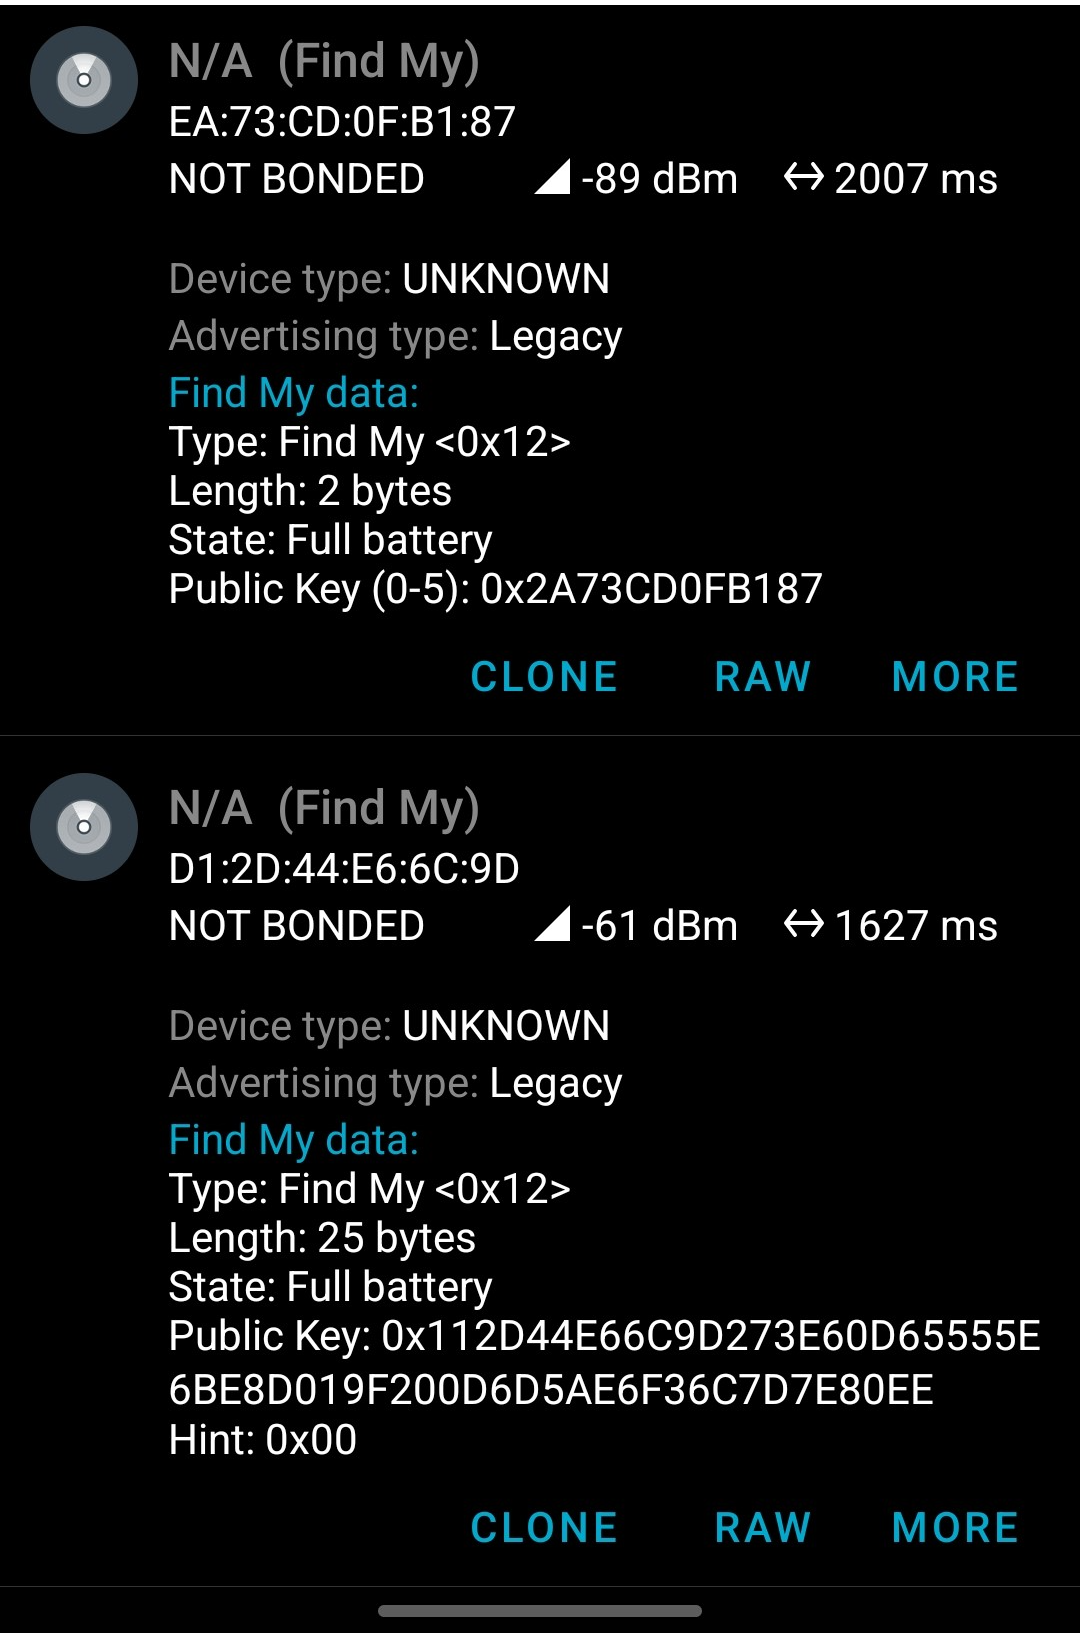
\includegraphics[height=8cm]{findMy_screenshot}
    \caption{Unterschiedliche Daten im Advertisement-Paket abhängig vom Zustand des Geräts.}
    \label{fig:findMy_screenshot}
\end{figure}

Sobald ein Gerät die Internetverbindung oder die \ac{BLE}-Verbindung zum Owner Device verliert, wird es als Lost Device angesehen.
Um in diesem Zustand von anderen Finder Devices gefunden werden zu können, beginnt das Lost Device den kompletten öffentlichen Teil von $AK_i$ in den Advertisement-Paketen zu senden \cite{Apple_FindMySpec}.
Der Screenshot eines \ac{BLE}-Scans mit der nRF-Connect App in \autoref{fig:findMy_screenshot} zeigt, wie sich die Inhalte der Advertisement-Pakete abhängig vom Gerätezustand unterscheiden.
Das erste mit „\textit{(Find My)}“ gekennzeichnete Gerät ist ein iPad, dass sich aufgrund einer vorhandenen Internetverbindung nicht im verlorenen Zustand befindet.
Das zweite so gekennzeichnete Gerät ist ein iPhone ohne Internetverbindung und gilt demnach als Lost Device, weshalb hier der gesamte öffentliche Schlüssel im Advertisement-Paket enthalten ist.

Ab iOS 15 werden zudem ausgeschaltete iPhones als Lost Devices angesehen und senden periodisch Advertisement-Pakete.
So kann ein Gerät zum Beispiel gefunden werden, wenn es sich aufgrund niedriger Akkuladung abschaltet oder es zum Beispiel bei einem Diebstahl abgeschaltet wird \cite{Classen_FindMy}.

Wie bereits bei den Grundlagen zu \ac{BLE} erwähnt werden Advertisement-Pakete für Apples proprietäre Dienste immer mit dem Typ manufacturer-specific data gesendet, sodass für den jeweiligen Dienst relevante Daten enthalten sein können \cite{Spec_BLE_5.3}.
Das proprietäre Advertisement-Format von Apple verwendet zur Unterscheidung der einzelnen Dienste ein Byte, welches den Typ des Dienstes kodiert.
Ein weiteres Byte gibt die Länge der folgenden Daten an \cite{Martin_continuity,Heinrich_FindMy}.
Darauf folgt ein Status-Feld, welches den ungefähren Akkustand in den Stufen \textit{„Full“}, \textit{„Medium“}, \textit{„Low“} und \textit{„Very Low“} enthält \cite{Mayberry_Tracking}.
Zusätzlich kodiert dieses Feld den Typ des Geräts, von welchem das Advertisement Paket stammt.
Dabei wird zwischen Apple Endgeräten (iPhone, iPad, MacBook), AirTags, Drittanbieterprodukten und Kopfhörern unterschieden \cite{Heinrich_AirGuard,Mayberry_Tracking}.

Zur Identifikation des Lost Device und zur Verschlüsselung der Standortdaten muss der aktuelle Advertising Key $AK_i$ übertragen werden.
Jeder Advertising Key wird dabei üblicherweise für 15 Minuten verwendet, um die Verfolgung des Geräts anhand der Advertising-Daten für Dritte zu erschweren.
Danach wird der nächste Advertising Key $AK_{i+1}s$ verwendet \cite{Heinrich_FindMy}.
Da für die Ableitung des nächsten Schlüssels der \ac{MBK} benötigt wird, kann ein Angreifer das Gerät nur schwer anhand der ausgesendeten Advertisement-Pakete verfolgen.
Im Vergleich zu Konkurrenzprodukten kann so die Privatsphäre der Nutzer besser geschützt werden.

Die Y-Koordinate des Schlüssels wird für den \ac{ECDH}-Schlüsselaustausch nicht benötigt und muss demnach nicht im Advertisement übertragen werden, was die zu übertragende Datenmenge auf die 28 Byte der X-Koordinate von $AK_i$ reduziert \cite{Heinrich_FindMy}.
Jedoch sind in Apples Advertisement-Format nach dem Status-Feld nur 24 Byte verfügbar.
Deshalb  wird zusätzlich die Advertising-Address des Advertisement Pakets zur Kodierung der X-Koordinate von $AK_i$ ausgenutzt \cite{Heinrich_FindMy}.
Die Advertising-Address kann zum Schutz der Privatsphäre laut \ac{BLE}-Spezifikation \cite{Spec_BLE_5.3} von der tatsächlichen \ac{MAC}-Adresse des Geräts abweichen.
Üblicherweise wird diese Funktion verwendet, um über zufällige \ac{MAC}-Adressen die Nachverfolgbarkeit von Geräten sowie Rückschlüsse auf den Gerätehersteller anhand der ersten drei Byte der \ac{MAC}-Adresse zu erschweren.
Durch Codierung von Daten in der zufälligen Adresse, kann das Feld jedoch für den Transfer beliebiger Daten ausgenutzt werden.
Apple sendet die ersten 46 Bit der X-Koordinate in der Advertising-Address, wobei die beiden \acp{MSB} des ersten Bytes jeweils auf 1 gesetzt werden müssen, um der \ac{BLE}-Spezifikation zu genügen \cite{Heinrich_FindMy}.
Die restlichen 170 Bit, bestehend aus den Bytes 6 bis 27 und den fehlenden zwei Bits des Byte 0 werden im Advertising Payload übertragen \cite{Apple_FindMySpec,Heinrich_FindMy}.
\autoref{fig:apple_advertising} zeigt den resultierenden Aufbau eines Advertisement Pakets des „Wo ist?“ Dienstes.
Die Teile, in welchen der öffentliche Schlüssel übertragen wird, sind gelb hinterlegt.
\begin{figure}[ht]
    \centering
    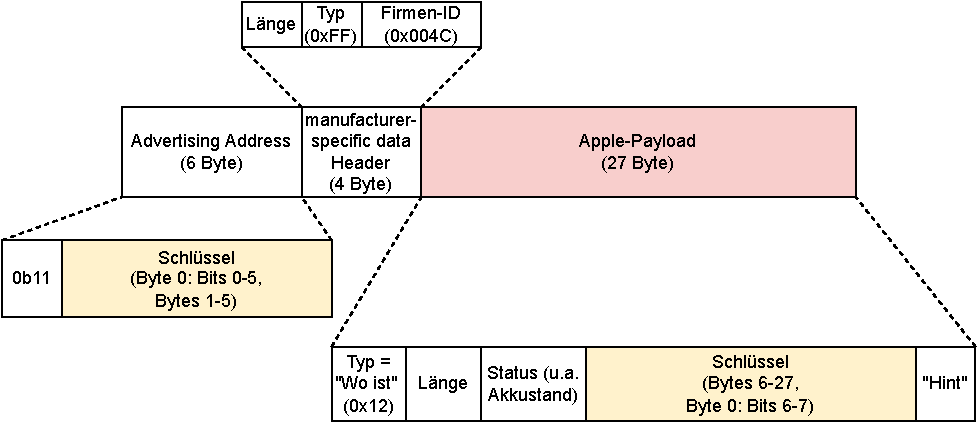
\includegraphics[width=0.9\textwidth]{apple_advertising.pdf}
    \caption{Aufbau der Advertisement-Pakete des „Wo ist?“ Dienstes.}
    \label{fig:apple_advertising}
\end{figure}
Das als "Hint" bezeichnete Feld kodiert laut Spezifikation \cite{Apple_FindMySpec} Byte 5 des öffentlichen Schlüssels, laut Heinrich \textit{et al.} \cite{Heinrich_FindMy} ist dieses Feld bei iOS allerdings immer 0.
Mayberry \textit{et al.} \cite{Mayberry_Tracking} konnten beobachten, dass dieses Feld bei AirTags tatsächlich auf Byte 5 des öffentlichen Schlüssels gesetzt wird, konnten aber keine weitere Funktion des Felds für den „Wo ist?“ Dienst identifizieren.
Da weder \cite{Heinrich_FindMy} noch \cite{Mayberry_Tracking} eine Funktion dieses Felds identifizieren können und die Spezifikation \cite{Apple_FindMySpec} keine weiteren Informationen zu diesem Feld enthält, wird angenommen, dass es aktuell keine Funktion erfüllt.

\subsubsection{Finden verlorener Geräte}
\label{sec:finden}
Standardmäßig scannen alle Apple-Geräte (Finder-Devices) im Hintergrund nach Advertisements, die die Firmen-ID von Apple enthalten \cite{Heinrich_FindMy,Martin_continuity}.
Wird ein Paket durch den Apple Payload Typ 0x12 als Advertisement für den „Wo ist?“ Dienst identifiziert, wird vom Finder Device zunächst die aktuelle Position bestimmt und ein Location Report erstellt.
Das Format dieses Reports ist in \autoref{fig:location_report} gezeigt.
\begin{figure}[ht]
    \centering
    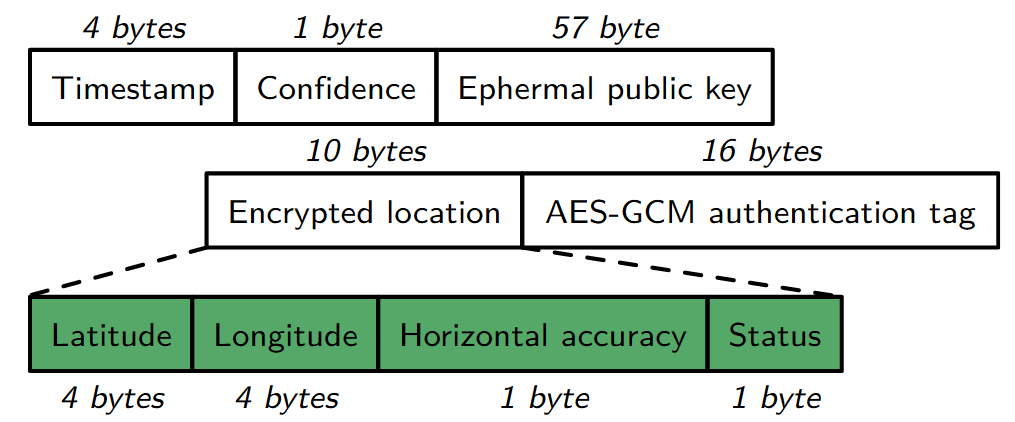
\includegraphics[width=0.85\textwidth]{location_report}
    \caption{Format des Location Reports \cite{Heinrich_FindMy}}
    \label{fig:location_report}
\end{figure}
Die Hauptbestandteile des Reports sind die verschlüsselten Standortinformationen, bestehend aus Koordinaten, Genauigkeit und Status.
Außerdem sind sowohl der öffentliche Teil des temporären Schlüssels $K_{ECC}'$, welcher vom Finder-Device für den \ac{ECDH}-Schlüsselaustausch genutzt wurde, und der \ac{AES}-\ac{GCM} Authentication Tag, Teil des Reports.
Zusätzlich ist ein Zeitstempel enthalten, der angibt, wann der Report erstellt wurde.
Dieser Report wird auf Apples Server hochgeladen und dabei mit einem \ac{SHA}-256 Hash der X-Koordinate von $AK_i$ verknüpft.
Dieser Hash wird benötigt, um die Zuordnung des Reports zu einem Lost Device und die Identifizierung des für die Verschlüsselung verwendeten $AK_i$ zu ermöglichen \cite{Heinrich_FindMy}.
Im Vergleich zu konkurrierenden Diensten sind die Verschlüsselung der Standortinformationen und die Pseudonymisierung durch den Hashwert wichtige Schritte, um Sicherheit und Privatsphäre des Dienstes zu verbessern.

In der Regel laden Finder Devices Location Reports nicht unmittelbar nach ihrer Erstellung hoch.
Stattdessen sammelt das Gerät mehrere Reports um diese später gebündelt hochzuladen.
Tonetto \textit{et al.} \cite{Tonetto_FindMy} zeigen, dass die Art der Internetverbindung beeinflusst, wann die Reports hochgeladen werden.
So liegt der Median für den Upload eines Reports bei aktiver WLAN-Verbindung bei 15 Minuten.
Ist keine WLAN-Verbindung, sondern nur eine Mobilfunkverbindung vorhanden, werden die Reports im Median erst nach 3 Stunden hochgeladen.

Der Upload erfolgt über einen HTTPS-Request, der über Informationen im HTTP-Header authentifiziert wird.
Der Header enthält unter anderem das Identitäts-Zertifikat des Geräts und eine Signatur des Requests.
Diese Signatur wird mit dem privaten Schlüssel erstellt, der in einem speziellen Sicherheitsbereich, dem \textit{Secure Enclave Processor} des Geräts gespeichert ist, welcher das unberechtigte Auslesen darin gespeicherter Daten verhindert.
Die Signatur kann demnach nur auf dem Gerät erfolgen.
Somit kann sichergestellt werden, dass nur Apple Geräte in der Lage sind Reports hochzuladen, was Apple vermutlich dazu nutzt, um das Erstellen gefälschter Reports zu erschweren \cite{Heinrich_FindMy}.
Der Server prüft die Signatur und die Authentifizierung des Geräts, ordnet den Reports den aktuellen Zeitstempel als Uploadzeitpunkt zu und speichert diese.

Um die Standortdaten vom Server abzurufen, sendet das Owner Device eine Anfrage mit einer Liste von Hashes der letzten Advertising Keys des Lost Device.
Diese Anfrage erfolgt ebenfalls über einen authentifizierten HTTPS-Request.
Die Authentifizierung erfolgt über die Apple-ID des Nutzers, sodass Apple jede Anfrage mit einem Nutzer verknüpfen kann.
Anhand der übermittelten Hashwerte kann der Server die zugehörigen Location Reports identifizieren und zurückgeben.

\autoref{lst:findmy_result} zeigt die Struktur der Antwort auf einen solchen Request in gekürzter Form.
Die Antwort besteht aus einem Array von Objekten, die jeweils den Hash des Advertising Keys (\textit{id}), den verschlüsselten Location Report (\textit{payload}) und Metadaten, darunter den Uploadzeitpunkt (\textit{datePublished}), enthalten.
\begin{lstlisting}[label=lst:findmy_result,caption={Beispielhafte Antwort beim herunterladen von Location Reports\cite{Heinrich_FindMy}.}]
{
    "results": 
    [
        {
            "datePublished": 1586804587284,
            "payload": "JETtmwIEzRBG ....",
            "description": "found",
            "id": "B6E5tpUPbuudAc ...",
            "statusCode": 0
        },
        ...
    ] ,
    "statusCode": "200"
}
\end{lstlisting}

Das Owner Device kann anhand des Hashwerts in jedem Report den für die Erstellung verwendeten Advertising Key identifizieren und den zugehörigen privaten Schlüssel verwenden, um den Schlüssel abzuleiten und die Daten zu entschlüsseln \cite{Heinrich_FindMy}.
Zur Steigerung der Genauigkeit bei der Positionsermittlung können die Informationen aus mehreren Location Reports eines Lost Devices miteinander kombiniert werden.
Bis zu sieben Tage nach dem Upload eines Location Reports kann dieser abgerufen werden.
Neuere Reports verhindern das Abrufen vorhandener nicht.
Die Kombination der Standorte der letzten sieben Tage kann genutzt werden, um den Pfad zu rekonstruieren, der vom verlorenen Gerät zurückgelegt wurde \cite{Heinrich_FindMy}.
